% ===========================================================================
%  pico-JEPA v2 --- presentacion para congreso (15 minutos)
%
%  Tema: UTN-BHI (https://github.com/javierip/custom-beamer). No se versiona
%  aqui: compile.sh lo clona y deja beamerthemeUTN-BHI.sty y theme/ junto a
%  este archivo (ambos en .gitignore). Formato 4:3, como el original: el
%  fondo institucional reserva la franja inferior para el logotipo.
%
%  Presupuesto de tiempo: 13 min de exposicion + 2 min de preguntas.
%  Cada diapositiva lleva un comentario con el tiempo previsto y una nota
%  para el orador (\note). Para verlas durante la charla, descomentar la
%  linea \setbeameroption de mas abajo y usar un proyector con dos pantallas.
% ===========================================================================
\documentclass[10pt]{beamer}

\usepackage[T1]{fontenc}
\usepackage[utf8]{inputenc}
\usepackage{microtype}
\usepackage[spanish,provide=*]{babel}
\usepackage{amsmath,amssymb}
\usepackage{graphicx}
\usepackage{booktabs}
\usepackage{url}
\usepackage{tikz}
\usetikzlibrary{arrows.meta, positioning, fit, backgrounds, calc}

\usetheme{UTN-BHI}

% Las figuras se toman del directorio del articulo: una sola copia de cada
% imagen en el repositorio. El segundo path permite tambien dejarlas aqui.
\graphicspath{{../paper/}{./figs/}{./}}

% El fondo institucional lleva el logotipo abajo y al centro. Una linea de
% pie vacia pero con altura le reserva esa franja al area de texto, para que
% ninguna diapositiva escriba encima.
\setbeamertemplate{footline}{\vspace{11mm}}

% El tema define el verde y el gris institucionales. Para el enfasis en
% cuerpo de texto hace falta una version mas oscura del verde: el original
% es muy claro sobre blanco.
\definecolor{greenUTNdark}{rgb}{0.42,0.44,0.0}
\setbeamercolor{alerted text}{fg=greenUTNdark}
\setbeamercolor{block title}{fg=white, bg=grayUTN}
\setbeamercolor{block body}{fg=grayUTN, bg=grayUTN!10}
\setbeamercolor{block title alerted}{fg=white, bg=greenUTNdark}
\setbeamercolor{block body alerted}{fg=grayUTN, bg=greenUTN!15}
\setbeamerfont{block title}{size=\small}
\setbeamerfont{frametitle}{size=\large, series=\bfseries}

% Diapositiva de seccion, como en la plantilla original.
\AtBeginSection[]{
  \begin{frame}
  \vfill
  \centering
  \begin{beamercolorbox}[sep=8pt,center]{title}
    \usebeamerfont{title}\insertsectionhead\par%
  \end{beamercolorbox}
  \vfill
  \end{frame}
}

% Notas del orador en una segunda pantalla (descomentar para presentar):
%\usepackage{pgfpages}
%\setbeameroption{show notes on second screen=right}

% Estilos de los diagramas, tomados del articulo. Las tipografias van un
% escalon mas grandes que alli: el diagrama se reescala al ancho del marco,
% de modo que un cuerpo mayor en el origen se proyecta mas legible desde el
% fondo de la sala.
\tikzset{
  dgm/.style={font=\sffamily\small,
              >={Latex[length=1.6mm]}, semithick},
  blk/.style={draw, rounded corners=2pt, align=center, inner sep=3pt,
              minimum height=9mm, minimum width=20mm},
  dat/.style={blk, fill=black!6},
  enc/.style={blk, fill=blue!10},
  prd/.style={blk, fill=orange!18},
  los/.style={blk, fill=green!14},
  sm/.style={font=\sffamily\scriptsize, inner sep=1.5pt, align=center},
  ar/.style={->}
}

\renewcommand{\arraystretch}{1.15}

% ---------------------------------------------------------------------------
\title[pico-JEPA v2]{pico-JEPA v2}
\subtitle{¿Cuándo superan muchos modelos pequeños a uno grande?}
\author[A. Rostagno et al.]{A.~Rostagno \and J.~Iparraguirre \and
                            R.~Briatore \and A.~González \and S.~Aggio}
\institute{Universidad Tecnológica Nacional\\
           Facultad Regional Bahía Blanca, Argentina\\
           \url{https://github.com/BHI-Research/pico-jepa-v2}}
% TODO: completar con el nombre, la sede y la fecha del congreso.
% \date{\itshape[Congreso --- sede y fecha]}

\begin{document}

% == Portada ============================================== ~0:30 ==========
\begin{frame}[plain]
  \titlepage
\end{frame}
\note{Presentarse y enunciar la pregunta en una frase: con un presupuesto
fijo, ¿un modelo grande o varios chicos? Anticipar que la respuesta es
«depende», y que el aporte es decir de qué depende.}

% == 1. El problema ======================================= ~1:15 ==========
\begin{frame}{Entender video sin etiquetas, en una PC de escritorio}
  \begin{itemize}
    \item Etiquetar video a mano es caro y lento.
    \item El aprendizaje \alert{auto-supervisado} aprende mirando video
          \alert{sin etiquetas}.
    \item \alert{JEPA} predice la región oculta \emph{en el espacio de
          representaciones}, no pixel a pixel: anticipa \emph{qué} hay, no
          lo dibuja.
    \item Nuestro escenario: una sola placa gráfica de escritorio
          (GTX 1060, 6\,GB).
  \end{itemize}

  \vfill
  \begin{block}{La pregunta de este trabajo}
    Con un presupuesto fijo de cómputo y datos, ¿conviene entrenar
    \alert{un único modelo} con todo el material, o \alert{varios modelos
    pequeños} ---cada uno con una porción--- y combinar sus predicciones?
  \end{block}
\end{frame}
\note{Insistir en el régimen: 6 GB de VRAM. Todo lo que viene está
condicionado por esa restricción, y es lo que hace interesante la pregunta
del reparto de datos.}

% == 2. De la v1 a la v2 ================================== ~1:15 ==========
\begin{frame}{De la v1 a la v2: de «funciona» a «cuándo funciona»}
  \small
  \textbf{pico-JEPA v1} (CACIC 2025): viabilidad en hardware de escritorio,
  con votación simple y pocas clases.

  \medskip
  La ventaja del conjunto \alert{no es automática}: depende de la capacidad
  de cada modelo, de la calidad de lo aprendido y de cómo se combinen las
  predicciones.

  \medskip
  \textbf{Qué agrega la v2:}
  \begin{enumerate}
    \item Un conjunto \alert{heterogéneo}: una cabeza de clasificación
          distinta por submodelo.
    \item El \alert{apilamiento}: un meta-modelo que aprende a quién
          conviene escuchar.
    \item Análisis estadístico formal, con intervalos de confianza.
    \item Un \alert{mapa de condiciones de validez}: cuándo aparece la
          ventaja y cuándo no.
  \end{enumerate}

  \vfill
  \begin{block}{}
    La pregunta interesante no es \emph{si} el conjunto gana, sino
    \emph{cuándo}.
  \end{block}
\end{frame}
\note{Esta es la bisagra de la charla: el aporte no es un número, es un mapa
de condiciones. Si hay que recortar tiempo, recortar después, no acá.}

% ===========================================================================
\section{Cómo funciona}
% ===========================================================================

% == 3. Etapa 1 =========================================== ~1:45 ==========
\begin{frame}{Etapa 1: aprender a representar, sin etiquetas}
  \centering
  \resizebox{\linewidth}{!}{%
  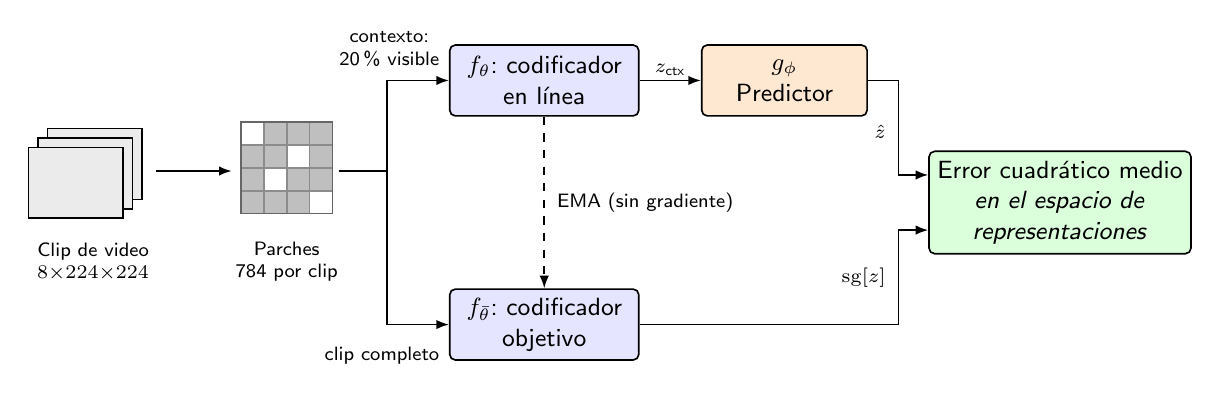
\begin{tikzpicture}[dgm]
    \foreach \o in {0.24, 0.12, 0} {
      \draw[fill=black!8] (\o,\o) rectangle ++(1.20,0.90);
    }
    \node[sm] at (0.82,-0.55) {Clip de video\\$8{\times}224{\times}224$};

    \begin{scope}[shift={(2.70,0.06)}, scale=0.29]
      \fill[black!25] (0,0) rectangle (4,4);
      \foreach \x/\y in {0/3, 1/1, 2/2, 3/0} {\fill[white] (\x,\y) rectangle ++(1,1);}
      \draw[black!45, step=1] (0,0) grid (4,4);
      \draw[black!60] (0,0) rectangle (4,4);
    \end{scope}
    \node[sm] at (3.28,-0.55) {Parches\\784 por clip};

    \node[enc, minimum width=24mm] (fon) at (6.55,1.75) {$f_\theta$: codificador\\en línea};
    \node[enc, minimum width=24mm] (ftg) at (6.55,-1.35) {$f_{\bar\theta}$: codificador\\objetivo};
    \node[prd, minimum width=21mm] (pred) at (9.60,1.75) {$g_\phi$\\Predictor};
    \node[los, minimum width=31mm, minimum height=13mm] (loss) at (13.10,0.20)
         {Error cuadrático medio\\\emph{en el espacio de}\\\emph{representaciones}};

    \draw[ar] (1.62,0.60) -- (2.58,0.60);
    \draw[ar] (3.94,0.60) -- (4.55,0.60) |- (fon.west);
    \draw[ar] (3.94,0.60) -- (4.55,0.60) |- (ftg.west);
    \node[sm, anchor=east] at (5.28,2.15) {contexto:\\20\,\% visible};
    \node[sm, anchor=east] at (5.28,-1.75) {clip completo};

    \draw[ar] (fon) -- node[sm, above] {$z_{\text{ctx}}$} (pred);
    \draw[ar] (pred.east) -- (11.05,1.75) |- ([yshift=3.5mm]loss.west);
    \node[sm, anchor=east] at (10.95,1.10) {$\hat{z}$};
    \draw[ar] (ftg.east) -- (11.05,-1.35) |- ([yshift=-3.5mm]loss.west);
    \node[sm, anchor=east] at (10.95,-0.75) {$\mathrm{sg}[z]$};

    \draw[ar, dashed] (fon.south) -- node[sm, right=1mm, pos=0.5]
         {EMA (sin gradiente)} (ftg.north);
  \end{tikzpicture}}

  \vfill
  {\footnotesize
  \begin{itemize}
    \item Se muestra el \alert{20\,\%} de los parches y se predice el
          \alert{80\,\%} oculto.
    \item El codificador objetivo es un promedio móvil del otro y nunca
          recibe gradiente: eso \alert{evita el colapso}.
    \item Codificador: ViT compacto, $d{=}192$, profundidad 8,
          \alert{3.4\,M de parámetros} (la mitad de un ViT-Small).
  \end{itemize}}
\end{frame}
\note{Recorrer el diagrama de izquierda a derecha en unos 40 segundos. El
punto que no puede faltar: la pérdida se calcula entre representaciones, no
entre pixeles, y el stop-gradient es lo que evita el colapso.}

% == 4. Etapa 2 y el conjunto ============================= ~1:30 ==========
\begin{frame}{Etapa 2: clasificar, y el conjunto de cuatro submodelos}
  \small
  \begin{columns}[T, onlytextwidth]
    \begin{column}{0.47\textwidth}
      \textbf{Clasificar}
      \begin{itemize}
        \item Sobre el codificador ya entrenado se agrega una \emph{cabeza}
              de clasificación.
        \item Tres tipos: \alert{lineal}, \alert{MLP} de dos capas y
              \alert{atencional}.
        \item El codificador puede quedar congelado o ajustarse finamente.
      \end{itemize}
    \end{column}
    \begin{column}{0.47\textwidth}
      \textbf{El conjunto ($N{=}4$)}
      \begin{itemize}
        \item Cada submodelo ve \alert{$1/4$} de los datos, equilibrado por
              clase.
        \item Se lo hace distinto a propósito: tipo de cabeza,
              congelado/fino, lr $\pm 30\,\%$, semilla y épocas $\pm 2$.
        \item El primero conserva la configuración base, como referencia.
      \end{itemize}
    \end{column}
  \end{columns}

  \vfill
  \begin{block}{}
    El objetivo no es que cada submodelo sea bueno, sino que
    \alert{se equivoquen de maneras distintas}: solo entonces combinarlos
    aporta algo.
  \end{block}
\end{frame}
\note{La diversidad se diseña, no se espera. Aclarar que todos comparten el
codificador: la diversidad vive en la cabeza. Es también una limitación, y
se retoma al final.}

% == 5. Formas de combinar ================================ ~1:00 ==========
\begin{frame}{Cuatro maneras de combinar las predicciones}
  \small
  \begin{enumerate}
    \item \textbf{Votación dura}: gana la clase más votada.
    \item \textbf{Votación blanda}: se promedian las probabilidades.
    \item \textbf{Votación ponderada}: más peso a los submodelos que mejor
          rindieron en validación.
    \item \textbf{Apilamiento} (Wolpert, 1992): una regresión logística
          recibe las probabilidades de todos y \alert{aprende} a quién
          conviene escuchar para cada clase.
  \end{enumerate}

  \vfill
  \begin{block}{La diferencia conceptual}
    Las tres votaciones aplican \alert{reglas fijas}; el apilamiento
    \alert{aprende la combinación a partir de los datos}. Esa diferencia
    resulta ser decisiva.
  \end{block}
\end{frame}
\note{Dejar planteado el suspenso: tres de estas cuatro van a perder contra
el modelo único. Sirve para que el resultado de la tabla se lea como
respuesta a una pregunta, no como una lista de números.}

% ===========================================================================
\section{Evaluación y resultados}
% ===========================================================================

% == 6. Configuracion y metrica =========================== ~1:30 ==========
\begin{frame}{Configuración y protocolo de medición}
  \footnotesize
  \begin{columns}[T, onlytextwidth]
    \begin{column}{0.48\textwidth}
      \textbf{Datos y cómputo}
      \begin{itemize}
        \item Kinetics-700-2020.
        \item Pre-entrenamiento: \alert{3\,000 videos sin etiquetas},
              20 épocas.
        \item Clasificación: \alert{30 clases}, 1\,467 videos
              $\rightarrow$ 876 / 297 / \alert{294 reservados}.
        \item 10 fragmentos por video al evaluar.
        \item Core i7, 65\,GB de RAM, GTX 1060 de 6\,GB.
      \end{itemize}
    \end{column}
    \begin{column}{0.48\textwidth}
      \textbf{La métrica: la brecha $\Delta$}
      \[
        \Delta = \text{exact}_{\text{conj}} - \text{exact}_{\text{únic}}
        \quad [\text{pp}]
      \]
      \begin{itemize}
        \item \textbf{Bootstrap}: $10\,000$ remuestreos $\Rightarrow$
              IC del 95\,\%.
        \item Veredictos fijados \alert{de antemano}:
          \begin{itemize}
            \item \textbf{SOPORTADO}: $\text{IC}_{\text{inf}} > 0$
            \item \textbf{INCONCLUSO}: $\Delta > 0$, el IC contiene el 0
            \item \textbf{RECHAZADO}: $\Delta \leq 0$
          \end{itemize}
      \end{itemize}
    \end{column}
  \end{columns}

  \vfill
  \centering
  El conjunto reservado permanece \alert{intocado} hasta la medición final.
\end{frame}
\note{Subrayar la disciplina metodológica: métrica y umbrales fijados antes
de mirar los datos, y el holdout se toca una sola vez. Es lo que da valor a
los números que siguen.}

% == 7. Nueve de nueve ==================================== ~1:15 ==========
\begin{frame}{Una señal consistente: nueve mediciones, nueve positivas}
  \centering
  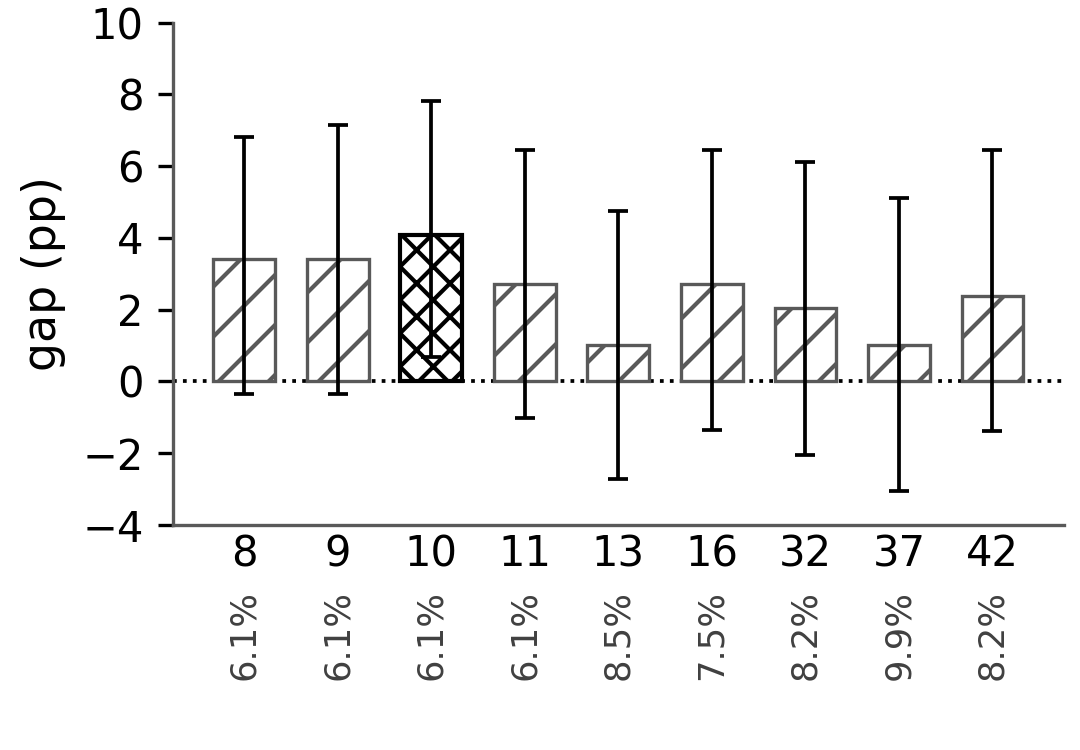
\includegraphics[width=0.88\linewidth]{fig1_phase4_timeline.png}

  \vfill
  {\footnotesize
  \begin{itemize}
    \item La exploración la condujo un \alert{bucle de experimentación
          automatizada}, con la métrica fijada de antemano.
    \item Nueve mediciones: \alert{las nueve positivas}, promedio
          $+2.53$\,pp. Si la brecha real fuera cero, sería tan improbable
          como nueve caras seguidas: $0.5^9 \approx 0.002$.
    \item \textbf{Cuidado}: comparten el conjunto reservado, así que son
          \alert{consistencia direccional}, no una prueba formal.
  \end{itemize}}
\end{frame}
\note{No sobrevender: decirlo explícitamente («esto todavía no es la prueba
formal; la prueba viene en la próxima diapositiva»). Es lo que un revisor
va a preguntar.}

% == 8. Resultado central ================================= ~1:30 ==========
\begin{frame}{El resultado central: solo el apilamiento gana}
  \centering
  \footnotesize
  \begin{tabular}{lcccc}
    \toprule
    \textbf{Combinación} & \textbf{Exactitud} & \textbf{Brecha}
      & $\text{IC}_{95\%}$ inf. & \textbf{Veredicto} \\
    \midrule
    \textbf{Apilamiento} & \textbf{11.90\,\%} & $\mathbf{+5.10}$\,pp
      & $\mathbf{+0.68}$ & \textbf{SOPORTADO} \\
    Votación dura        & 8.84\,\% & $+2.04$\,pp & $-1.70$ & INCONCLUSO \\
    Votación blanda      & 8.50\,\% & $+1.70$\,pp & $-2.04$ & INCONCLUSO \\
    Votación ponderada   & 7.48\,\% & $+0.68$\,pp & $-2.72$ & INCONCLUSO \\
    \bottomrule
  \end{tabular}

  \medskip
  Experimento controlado: se fijan los submodelos y el modelo único
  (\alert{6.80\,\%}) y solo cambia la forma de combinar.

  \vfill
  \begin{block}{}
    El apilamiento es la \alert{única} estrategia cuyo intervalo excluye el
    cero. Las tres votaciones simples quedan \alert{por debajo} del modelo
    único en exactitud absoluta.
  \end{block}
\end{frame}
\note{Dar tiempo a que se lea la columna del IC inferior. El dato
contraintuitivo, y el que más se comenta después, es que las votaciones
pierden contra el modelo único.}

% == 9. Lectura del resultado ============================= ~1:15 ==========
\begin{frame}{La diversidad no alcanza: hay que aprender a combinarla}
  \centering
  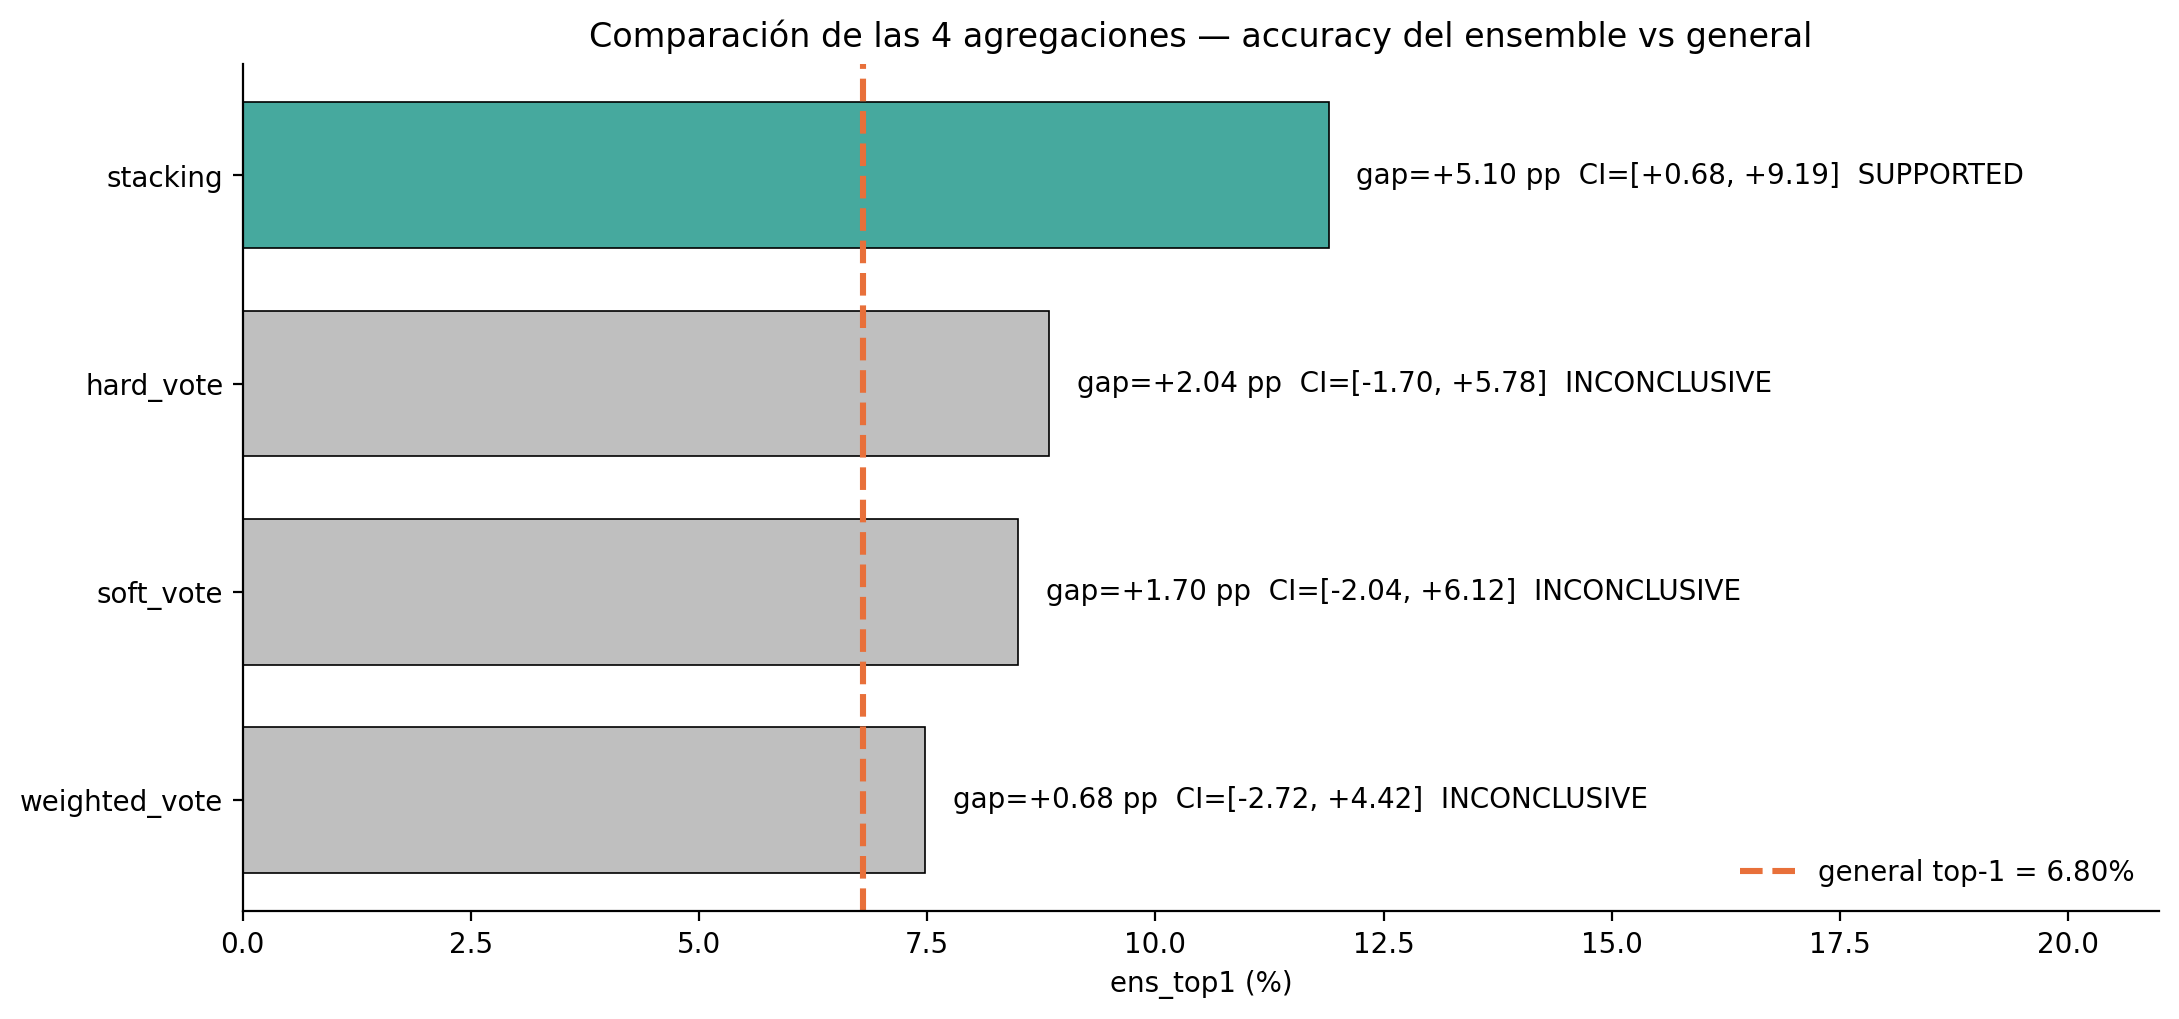
\includegraphics[width=0.78\linewidth]{fig2_aggregations.png}

  \vfill
  {\footnotesize
  \begin{itemize}
    \item Promediar a ciegas las predicciones de submodelos que vieron pocos
          datos \alert{perjudica el resultado}, salvo que un meta-modelo
          aprenda cuándo conviene escuchar a cada uno.
    \item Con Bonferroni ($\alpha = 0.0125$) el
          $\text{IC}_{\text{inf}} = +0.68$\,pp es \alert{marginal}: la
          solidez viene de tres líneas de evidencia convergentes.
    \item Con cuatro semillas independientes el $\text{IC}_{\text{inf}}$ se
          mantuvo positivo en los cuatro casos ($+0.68$ a $+1.02$\,pp).
  \end{itemize}}
\end{frame}
\note{Honestidad estadística: decir en voz alta que bajo Bonferroni el
resultado es marginal, y que por eso se apoya en la convergencia de las
nueve mediciones y los dos experimentos controlados.}

% ===========================================================================
\section{Los límites de la ventaja}
% ===========================================================================

% == 10. Cuando no funciona =============================== ~1:30 ==========
\begin{frame}{¿Cuándo no funciona? Dos experimentos controlados}
  \centering
  \footnotesize
  \begin{tabular}{lcccc}
    \toprule
    \textbf{Variante} & $d$ & Clases & $\Delta$ & \textbf{Veredicto} \\
    \midrule
    \textbf{Principal} & \textbf{192} & \textbf{30} & $\mathbf{+5.10}$\,pp
      & \textbf{SOPORTADO} \\
    Menor capacidad & 128 & 30 & $+0.00$\,pp & RECHAZADO \\
    Pocas clases    & 192 & 10 & $-1.50$\,pp & RECHAZADO \\
    \bottomrule
  \end{tabular}

  \vfill
  \raggedright
  {\footnotesize
  \begin{itemize}
    \item \textbf{Menor capacidad:} el modelo único incluso mejora
          (11.6\,\%), pero la brecha cae exactamente a cero, con un IC
          degenerado $[-0.04,\,+0.04]$.
    \item \textbf{Pocas clases:} concentrar los datos fortalece al modelo
          único (22.5\,\%) y la brecha se vuelve negativa.
  \end{itemize}}

  \vfill
  \begin{block}{}
    Mismo mecanismo en los dos casos: sin capacidad o sin variedad de
    clases, los submodelos \alert{convergen a la misma solución} y no queda
    diversidad que combinar.
  \end{block}
\end{frame}
\note{Este es, para nosotros, el aporte más útil del trabajo: publicar
también las condiciones en las que la idea falla. Decirlo con esas palabras.}

% == 11. Brecha vs. modelo unico ========================== ~1:00 ==========
\begin{frame}{La ventaja se achica cuando el modelo único mejora}
  \centering
  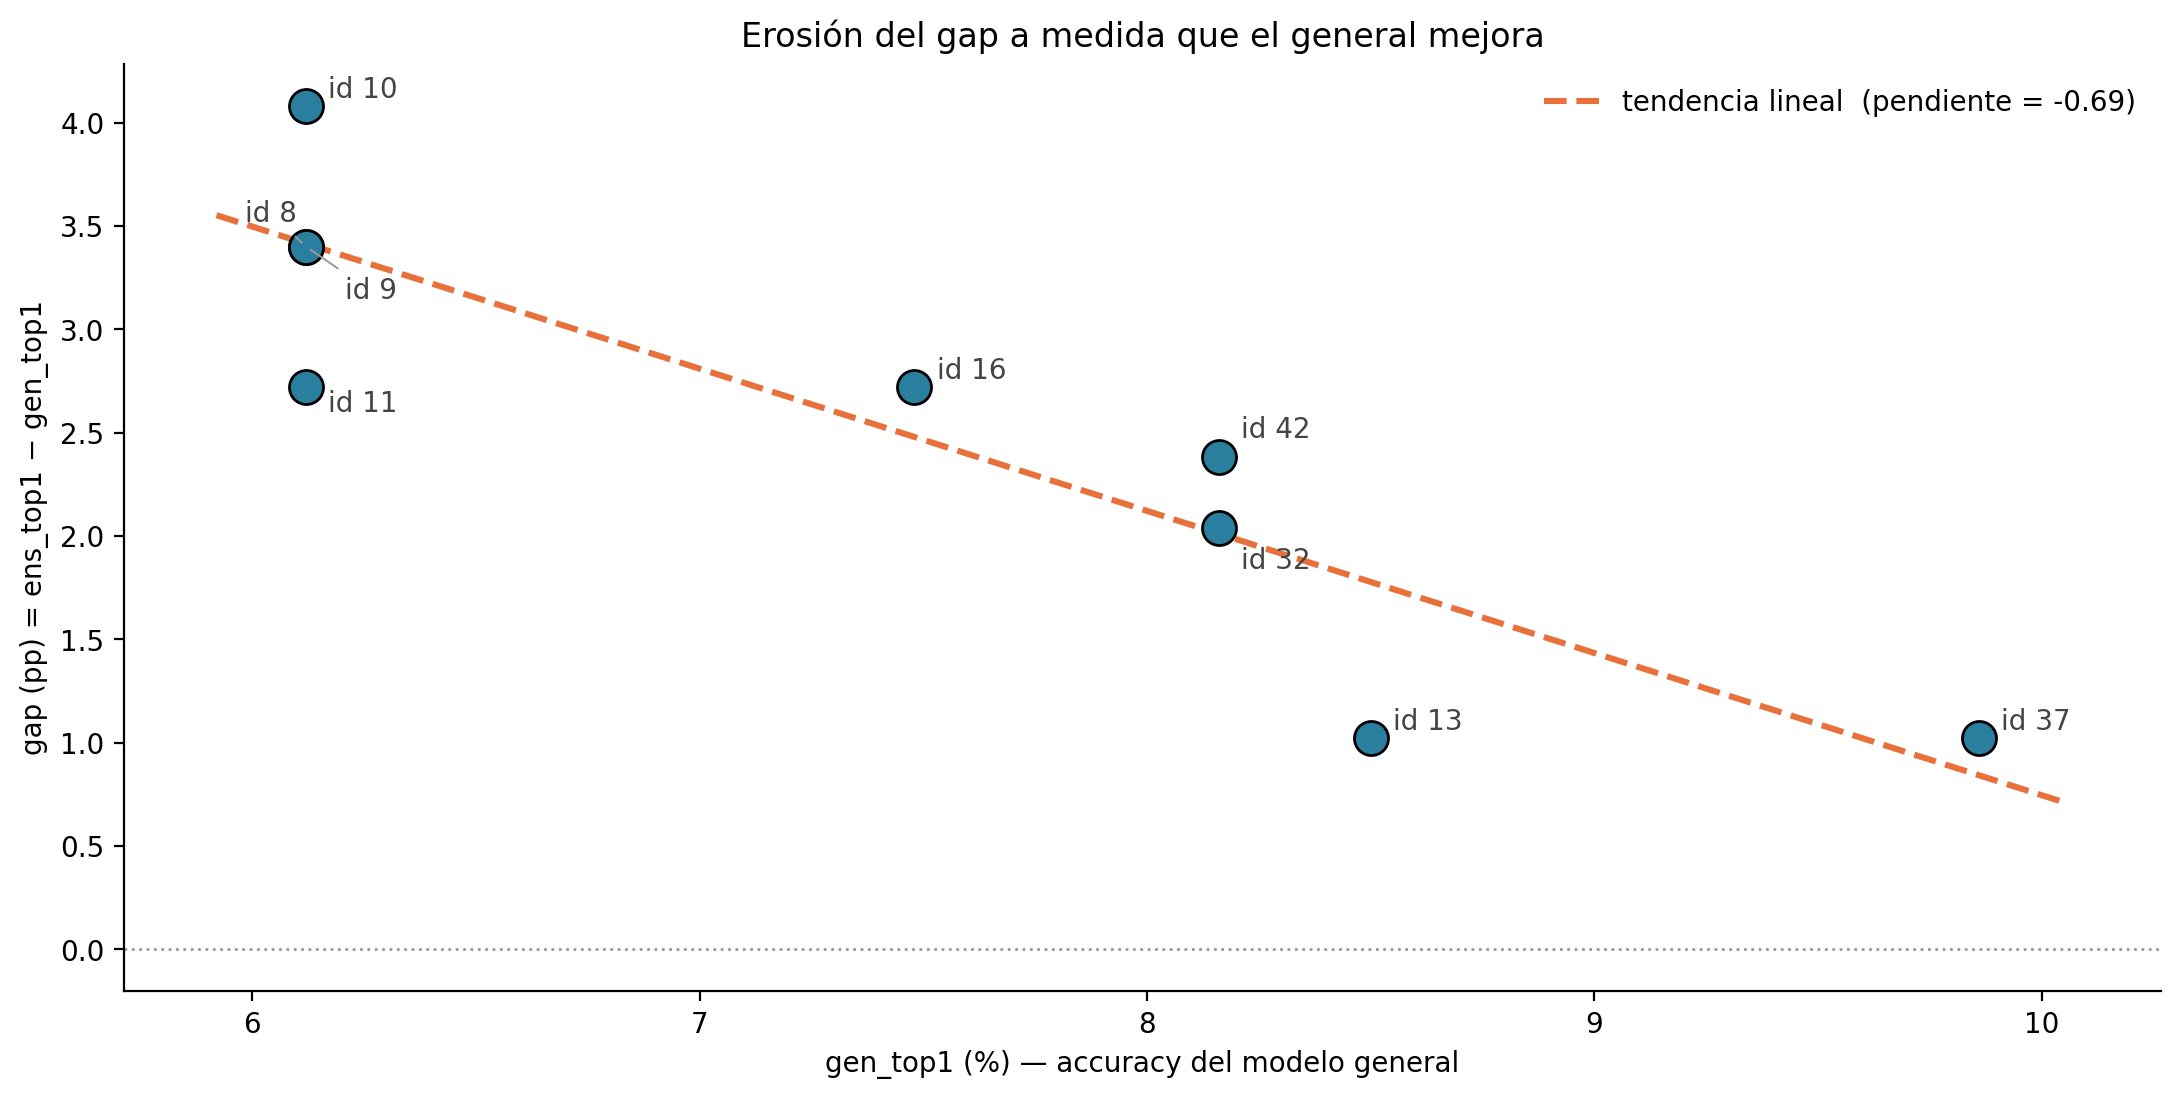
\includegraphics[width=0.78\linewidth]{fig3_gap_vs_general.png}

  \vfill
  \raggedright
  {\footnotesize
  \begin{itemize}
    \item A lo largo de las nueve mediciones la brecha se reduce a medida
          que el modelo único mejora
          (pendiente $\approx -0.69$, $R^2 \approx 0.80$).
    \item El modelo único ve \emph{todos} los datos: la ventaja del conjunto
          es más notoria cuando los modelos individuales son
          \alert{relativamente débiles}.
    \item Relación \alert{observacional} sobre nueve configuraciones: es una
          tendencia, no un efecto causal.
  \end{itemize}}
\end{frame}
\note{Si se va el tiempo, esta es la diapositiva a acortar: basta con la
pendiente negativa y la advertencia de que es observacional.}

% == 12. Limitaciones ===================================== ~1:00 ==========
\begin{frame}{Limitaciones}
  \small
  \begin{enumerate}
    \item El conjunto reservado es chico (\alert{294 videos}): los
          intervalos de cada medición individual son anchos.
    \item Las exactitudes absolutas son bajas (${\approx}12\,\%$ sobre 30
          clases, unas 3.6 veces el azar): el codificador se entrenó con
          solo 3\,000 videos, \alert{unas 670 veces menos} que el V-JEPA
          original.
    \item La diversidad se limita a la cabeza de clasificación: todos los
          submodelos \alert{comparten el codificador}, porque entrenar
          varios excedía la capacidad del hardware.
    \item Los resultados provienen de un \alert{único entrenamiento} del
          codificador: la variabilidad por inicialización queda fuera de los
          intervalos.
  \end{enumerate}
\end{frame}
\note{No leerlas todas: mencionar la 1 y la 3, que son las que suelen
preguntar, y dejar las otras en pantalla.}

% == 13. Conclusiones ===================================== ~1:15 ==========
\begin{frame}{Conclusiones}
  \small
  \begin{itemize}
    \item Hipótesis \alert{validada con significancia formal}
          ($\Delta = +5.10$\,pp, IC 95\,\% $[+0.68,\, +9.19]$), pero solo
          con \alert{diversidad}, \alert{apilamiento} y evaluación sobre
          múltiples fragmentos.
    \item Dos experimentos controlados marcan los límites: la ventaja se
          anula con menor capacidad ($d{=}128$) o con pocas clases
          ($C{=}10$).
    \item \textbf{Trabajo futuro}: más videos sin etiquetas para liberar el
          techo de la clasificación, y caracterizar cómo cambia la brecha al
          variar la cantidad de clases y la dimensión $d$.
  \end{itemize}

  \vfill
  \begin{block}{El mensaje práctico, para quien trabaje con recursos acotados}
    Dividir los datos entre varios modelos pequeños \alert{puede ganar,
    pero no gratis}: hay que diseñar la diversidad, aprender la combinación
    y verificar que el problema tenga espacio suficiente para que esa
    diversidad exista.
  \end{block}
\end{frame}
\note{Cerrar con la frase «puede ganar, pero no gratis». Es la que conviene
que se lleven.}

% == Cierre =============================================== ~0:15 ==========
\begin{frame}
  \begin{center}
    \begin{beamercolorbox}[sep=8pt,center]{title}
      \usebeamerfont{title}\Large{¡Gracias!}
    \end{beamercolorbox}
    \vspace{1em}
    \huge{¿Preguntas?}\\
    \vspace{1.5em}
    \small{\url{https://github.com/BHI-Research/pico-jepa-v2}}
  \end{center}
\end{frame}

\end{document}
